\documentclass[10pt,a4paper]{scrartcl}

\usepackage[utf8x]{inputenc}
\usepackage{ucs}
\usepackage{amsmath}
\usepackage{amsfonts}
\usepackage{amssymb}
\usepackage{subfig}
\usepackage{graphicx}
\usepackage[british]{babel}

\setlength{\parskip}{0.5em}


\title{Sputnik}
\subtitle{Project Report HCC Project Seminar 2011}
\author{Simon Wallner\footnote{\texttt{me@simonwallner.at}}}

\begin{document}
\maketitle

\begin{abstract}
This paper evaluates \emph{Sputnik} a 3D environment with which the user can freely interact through an elastic \emph{arc of light/fishing rod} metaphor, to explore, create and interact with virtual \emph{sound objects}. These sound objects are placed in the scene and react to the user's input by sending MIDI commands to an external audio program thus creating or manipulating the sound.

\end{abstract}

\section{Reading Guide}
Appendices
Code
Prerequisitions
Video
CD
etc...


\section{Introduction}

% setting the scene
Computer music is around us for some time now and through the use of the computer musicians have sheer endless possibilities of musical expression. With this plethora of possibilities comes the need for constraints and control to harness this expressive potential. Over the recent years many standard and non-standard interface have been developed, ranging from the ordinary button-fader-nob MIDI interface to more elaborate interfaces and systems like the \emph{reactable}\cite{Jorda2007}, \emph{mixiTUI}\cite{Pedersen2009} or commercial solutions like the \emph{Novation Launchpad}\footnote{\texttt{http://www.novationmusic.com/products/midi\_controllers/launchpad}} or \emph{Native Instruments Maschine}\footnote{\texttt{http://www.native-instruments.com/\#/en/products/producer/maschine/}} to name but a few.

With the advent of motion based controllers in consumer entertainment systems, marked by the release of the \emph{Wii}\footnote{\texttt{http://de.wikipedia.org/wiki/Wii}} console in late 2006, motion controllers became widely and cheaply available. This and their interface capabilities make them the ideal tools to explore the realm of \emph{new interfaces for musical expression}.


% problem statement
A common problem of computer music interfaces is that often the process of sound creation is not readily comprehensible. Seeing a performer on stage behind their laptop twisting knobs and adjusting faders might be ambiguous to an uninformed observer. It can be hard to relate the artist's action to the resulting sounds. This can hinder the experience and might go as far as to the point where the audience suspects that an artist just pressed play, as interviews conducted by \cite{Pedersen2009} show.

% Sputnik description
This paper introduces \emph{Sputnik}, a system that uses a \emph{Wiimote} controller to interact with a dynamic 3D scene. In the scene, a variety of sound creating objects are placed that send MIDI signals to an external audio program upon the user's interaction. 

Users can freely navigate the 3D scene and interact with it through an elastic \emph{arc of light/fishing rod} metaphor. It seems as if the \emph{arc of light} was coming out of the Wiimote and reaches into the scene, acting as an extension of the user's body into the virtual space. With this bodily extension users can \emph{grab} and \emph{drag} objects around the 3D scene.



% contribution
In this paper I evaluate the qualities of the \emph{arc or light} metaphor and how the design decisions/constraints of the system influence its expressive potential both visually and musically. This evaluation is grounded in a user study of XXX users.

Based on these findings and the theoretical framework of \cite{Ullmer2000} the similarities and differences between \emph{Sputnik} and tangible user interfaces are discussed. 


\section{Paper Outline}
The following section gives an overview over related work in the field of \emph{New Interfaces for Musical Expression} and tangible user interfaces. Section \ref{sec:results} goes into detail about Sputnik, both on a conceptual and a technical level. Section \ref{sec:evaluation} describes the performed user study and the paper is finally concluded in section \ref{sec:discussion} where the findings are discussed.


\section{Related Work}
\paragraph{Practical Work}
Only a few projects exist that go into a similar direction as Sputnik. The \emph{Virtual Xylophone}\cite{Maki-Patola2005} is a virtual reality system in which the user can place xylophone bars of different pitch in the scene and then struck them with a virtual mallet. By translating the configuration and mapping of the real instrument into the VR environment, new modes of play emerge.
\cite{Zappi2010} created a virtual controller for \emph{Ableton Live} that allows users to create simple proxy objects in a VR environment, bind them to certain controls and use them effectively as virtual sliders. \cite{Rodet2005} created a virtual environment for an exhibition setting. Users interact with the system via a 6-DOF motion tracker with tactile feedback. However, the user's actions in the system are highly constrained.

More projects can be found in the realm of Tangible User Interfaces. With \emph{mixiTUI} \cite{Pedersen2009} created a table top tangible interface for a sequencer that aimed not only to be functional but also to visually enrich the artists performance. Interviews with musicians and an extensive user study have been performed. \cite{Jorda2007} created the famous \emph{reacTable}, also a table top tangible interface that allows the creation and manipulation of music by composing various objects on its surface. 

After the release of the Wii in late 2006, the Wiimote motion controller received some attention in and outside the field of musical interfaces: 
\cite{Kiefer2008} assess the general qualities of the Wiimote as a musical controller and \cite{Miller2010} uses the Wiimote and sensor bar to create the \emph{Wiiolin}, a virtual violin that mimics the real instrument and can be played either in an upright position like a cello or horizontally like a violin. It senses the button presses and tracks the movement of the \emph{bow}, i.e. the sensor bar to create the sounds.

Not a Wiimote but still impressive, \cite{Miyama2010} uses an low resolution distance sensor array to control the many parameters of a synthesizer. A small gui application is merely used for monitoring the system's state, and sound creation is done in pd.


\paragraph{Theoretical Work}
The field of \emph{Tangible User Interfaces (TUI)} provides part of the theoretical background for this work. Work of \cite{Fitzmaurice1995} and then later \cite{Ishii1997} introduced this term and the wider concept. \cite{Shaer2009} Gives a very good overview over this field as well as the history of TUI studies. \cite{Ullmer2000} introduced \emph{MCRpd}, a formal model for describing and analysing TUIs that will be used in section \ref{}.

\cite{Sharlin2004} introduced \emph{spacial TUIs} that focuses on \emph{I/O unification} by tightly coupling the action and perception spaces and embodying a clear state representation across all sensory modalities.


Entering the musical realm \cite{Fels2011} give a good overview and general introduction into the field of \emph{NIMEs (New Interfaces for Musical Expression)}. \cite{Cook2001} shares 13 general principles for designing computer music controllers that resulted from his long lasting experience in this field. \cite{Dobrian2006} asks the question of virtuosity and expression by pointing out the elephant in the room, e.g. the lack thereof and also the lack of a comparable standard repertoire. 

In contrary to that \cite{Gurevich2007} question the hegemonic \emph{composer--interpret--listener} relation in favour of a more holistic \emph{ecological} view of musical expression. Later work by \cite{Gurevich2010} evaluated a highly constrained, prototypical one-button instrument that spurred a wide variety of play styles in test users.

Closing the loop to design and HCI, \cite{Magnusson2010} gives a good overview over the field of \emph{affordance} and elaborates on \emph{contraints} from different viewing angles and how they impact and support creativity. Finally, \cite{Wanderley2002} goes into depth over evaluating input devices for musical expression in the context of HCI. 






% ------------------------------------------------

% \cite{Magnusson2010} gives a good overview over the field of \emph{affordance} and elaborates on \emph{constraints} from different viewing anlges and how constraints impact and support creativity.

% \cite{Ullmer2000} introduces a formal model for tangible user interfaces and compares it to the prevalent MVC (Model View Controller) model. Different qualities of TUIs are stated and a few existing applications are assessed with it.

% \cite{Ishii1997} Introduced the term \emph{Tangible User Interface} (\emph{TUI}

% \cite{Kiefer2008} Assessing the potential of the wiimote as an musical interface and comparing it to a common interface. user study, only very simple mapping + perceptron shape recognition

% \cite{Wanderley2002} discusses the problems of how to assess interfaces for musical expression and searches the depths of HCI studies for a possible answer. no answer given

% \cite{Dobrian2006} tries to answer what constitutes an expressive musical interface, and how does the lack of virtuoso performers impacts the whole discussion. It highlights the role of a repertoire and the role of the performer. This is a bit contradicting to what \cite{Magnusson2010} writes.

% \cite{Cook2001} provides a few (empiric) design principles for digital musical instruments and richly illustrates them with example projects.

% \cite{Fels2011} General introduction and overview to/of the field of NIMEs given as a SIGGRAPH course. The definitive introduction to NIMEs.

% \cite{Gurevich2007} introduce an \emph{ecological} view of musical expression that goes against the conservative view of a uni-linear composer--interpret--listener relation.

% \cite{Gurevich2010} evaluate a highly constrainted one-button instrument in terms of the style and variations these constraints induce.

% \cite{Maki-Patola2005} built four virtual reality instruments for a cave like environment, one of them being a virtual mallet, where users can hit the pads with virtual mallets. This comes closest to Sputnik and also a few general thought on virtual scenes and the possible impact on the performance are given.

% \cite{Miller2010} uses the Wiimote and sensor bar to modell a virtual violin. It has no graphical UI and uses recorded sound samples.

% \cite{Miyama2010} IR distance sensor array used to control a pd patch and a simple gui application written in c.

% \cite{Pedersen2009} mixiTUI, tangible sequencer with gui, user study and interviews.

% \cite{Sharlin2004} introduces \emph{spatial TUIs} and discusses I/O unification on a few examples, coupling of action and perception space.

% \cite{Fitzmaurice1995} introduces \emph{graspable user interfaces} with Briks.

% not used
% \cite{Gamberini2011} introduces \emph{action breakdowns} for quantitative studies of user interfaces.

% \cite{Shaer2009} Give a general introduction into the field of TUIs and provide an historical overview.

% furhter research
% \cite{Godoey2006} explores the the playing of \emph{air instruments} and what is behind it. 

% \cite{Zappi2010} built a motion tracked 3d virtual environment in which users can create/bind/interact with basic virtual objects to control all aspects of a \emph{live} set. Input done via hand gestures only simple parameter mapping, virtual faders.

% \cite{Rodet2005} haptic feedback to objects in a ve, very simple interaction, no direct scene interaction.






\section{Results}
\label{sec:results}
7-10 pages

Description of the Implementation according to the learning goals:


% Create a system that allows the user to interact with an virtual world through the Wiimote. This system should be intuitive even for untrained users, and have a very low barrier of entry.
% Explore the technical capabilities of the Wiimote and Nunchuck controller and put it to good use.
% Create a meaningful mapping form the virtual world to the sound generation system.
% Create a sound generation system that allows nuanced and rich musical expression.
% Develop an architecture that streamlines the three stages input - processing - output.


\subsection{Sputnik Overview}
% user domain description of Sputnik
% what is Sputnik in the user domain. Everything that is not technical or theoretical. This sets up the frame for alle the following section.

\emph{Sputnik} is a \emph{New Interface for Musical Expression} that combines 3D graphics with the capabilities of the Wiimote controller. The user is presented with colourful 3D scene that contains various simple objects. The user can freely navigate this scene and interact with these object to create sounds.

The user can interact with the system via a Wiimote and Nunchuck controller. The Nunchuck controls the users movement in the 3D space and the Wiimote is used to control the camera and to interact with the objects in the scene. 

\subsubsection{Setup}
The system is set up in a room with an overhead mounted video beamer. The sensor bar can either be placed on the upper or lower edge of the projected image. It consists of two IR emitters that allows the IR camera in the Wiimote to track its relative orientation in space. A Wiimote and Nunchuck controller are used and only a single person at a time can use the system. Figure \ref{fig:sputnik-setup} illustrates the setup.

\begin{figure}[hbtp]
\begin{center}
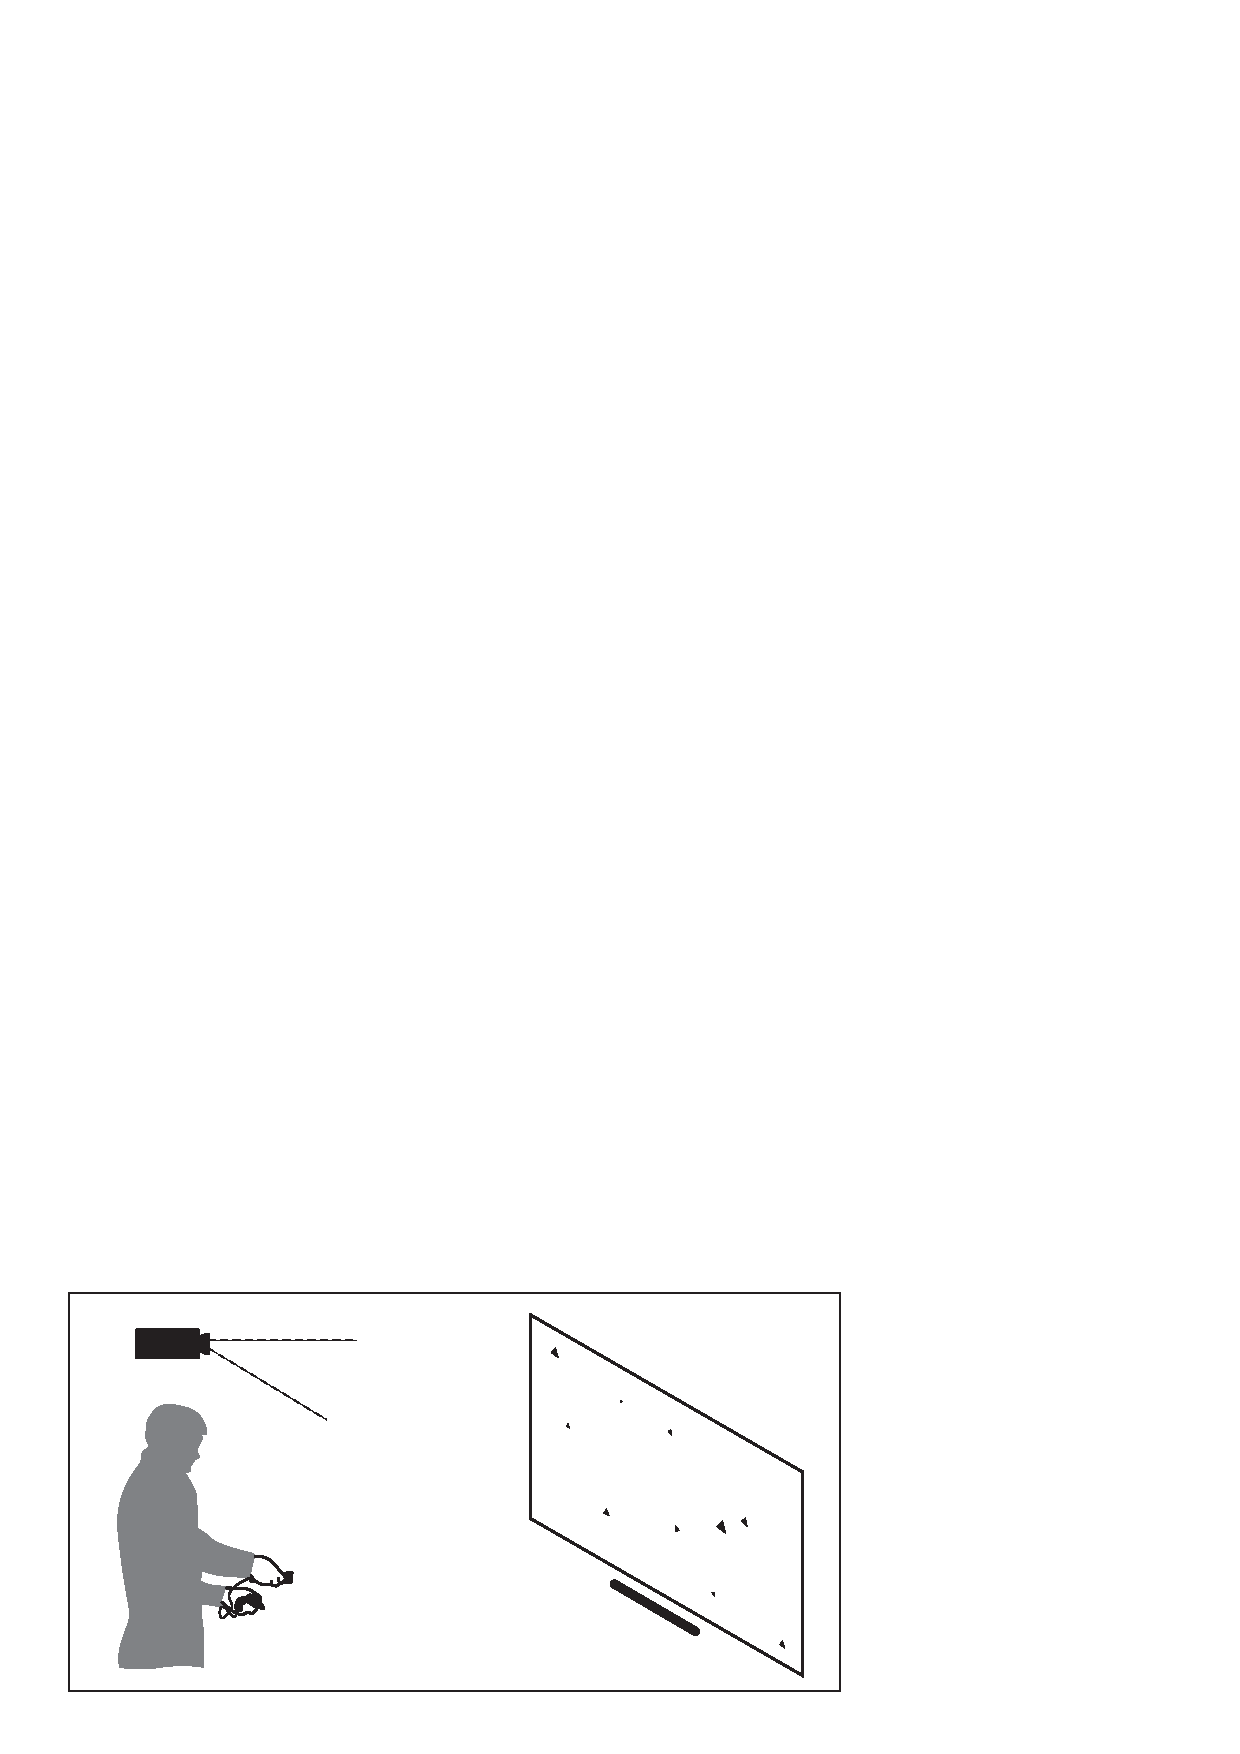
\includegraphics[width=0.4\columnwidth]{img/setup}
\caption{Standard set up of Sputnik}
\label{fig:sputnik-setup}
\end{center}
\end{figure}



\subsection{Navigation and Camera Controls}
Sputnik's virtual scene uses a fixed up direction and the user can move through the scene by pushing the Nunchuck's analogue stick in the respective direction. Pushing the stick forward moves the camera into the scene, pushing it left moves the camera to the left and vice versa.

Tilting and panning is controlled by pointing the Wiimote to the top/bottom/left/right of the screen. The farther it is pointed away from the neutral center position the faster the camera movement is. Figure \ref{fig:sputnik-navigation} illustrates the navigation.

\begin{figure}[hbtp]
\begin{center}
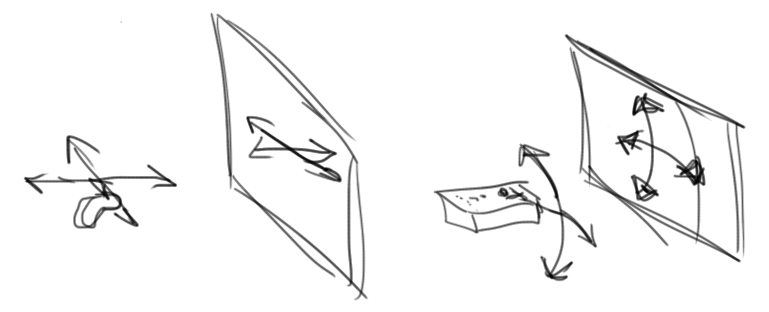
\includegraphics[width=0.7\columnwidth]{img/navigation}
\caption{The Nunchuk's analogue stick controls the camera's dolly and track movements, the Wiimote's IR pointer controls the camera's tilt and pan movements.}
\label{fig:sputnik-navigation}
\end{center}
\end{figure}




\subsubsection{Interaction}

\begin{figure}[hbtp]
\begin{center}
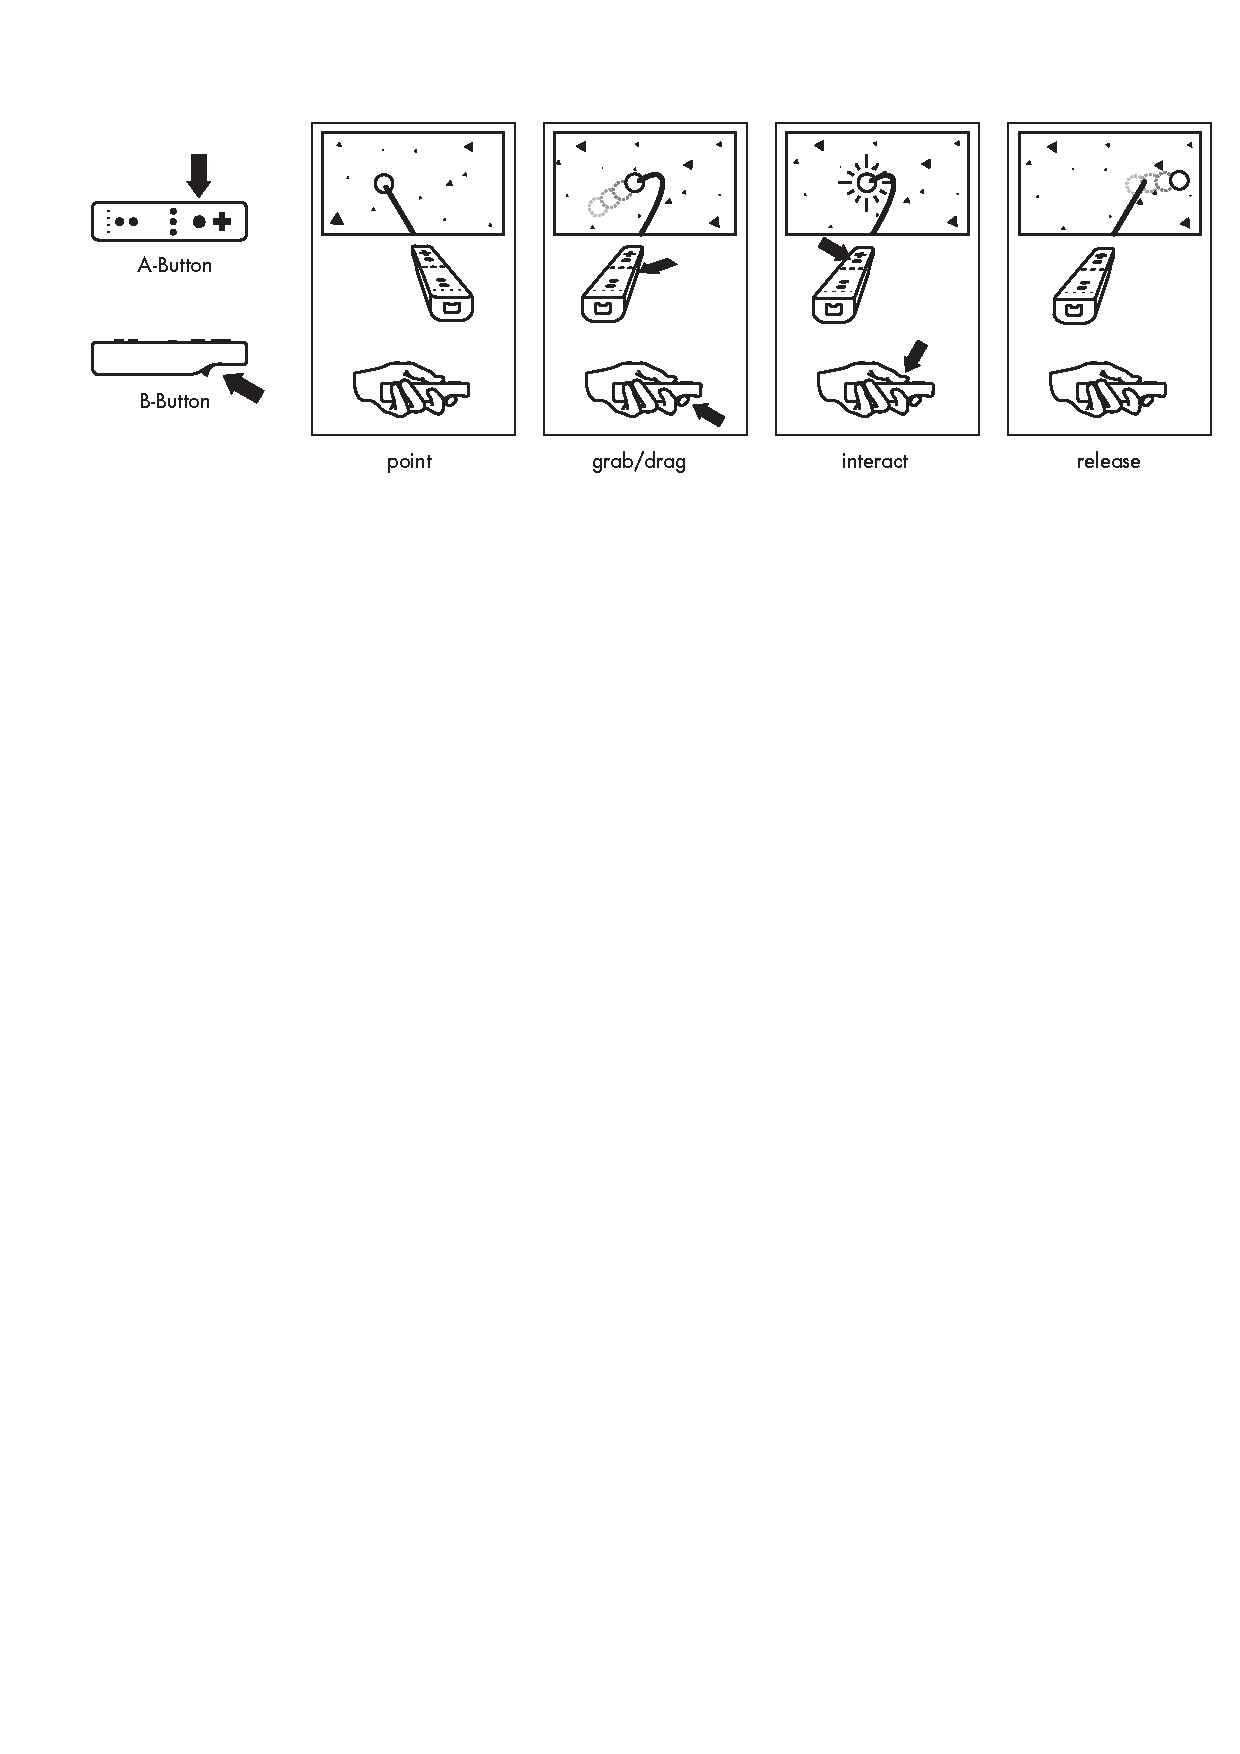
\includegraphics[width=0.95\columnwidth]{img/sputnik-overview}
\caption{The basic interaction vocabulary of Sputnik}
\label{fig:sputnik-overview}
\end{center}
\end{figure}

Figure \ref{fig:sputnik-overview} illustrates the basic interaction vocabulary of Sputnik. The user can interact with the scene via an \emph{arc of light metaphor}. It seems as if the arc of light was coming out of the Wiimote and reaches into the scene, acting as a bodily extension of the user into the virtual space. Through this \emph{arc} objects in the scene can be \emph{pointed} at, \emph{grabbed} and \emph{dragged} around as well as \emph{released}.

Objects behave in a simplified yet physically plausible way, each featuring distinct weight and friction. Dragging objects causes the arc to bend like a fishing rod, reflecting the physical properties of the object.

Each object in the scene can react individually to user interaction. The following classes of objects exist in Sputnik:
\begin{description}
\item[Sampler (red sphere)] The \emph{sampler} object reacts to the press of the \emph{A Button} while it is grabbed. While the button is held the sample is played in a loop and stops immediately when the button or the object is released. Playback always starts at the beginning of the sample.

\item[Player (yellow sphere)] The \emph{player} object reacts to the press of the \emph{A Button} while it is grabbed. Pressing the \emph{A button} starts and stops the player. It is not automatically stopped when it is released. Playback is looped and always starts at the beginning.

\item[Tape Machine (grey sphere)] Modelled after an old tape machine and inspired by \emph{musique concrète} the \emph{tape machine} object controls the speed of the play back by the object's movement speed in the virtual space. The faster it moves the faster the playback. Playback is looped.

\item[Harmonic Harp (orange spheres)] The orange spheres form a kind kind \emph{harmonic harp}. Each sphere controls a single sine wave oscillator and the volume is determined by the the spheres distance to is origin. Additionally a force exists that drags the spheres towards their respective origins. The oscillators are tuned to the natural harmonic series.
\end{description}

By interacting with the different objects and arranging the in the virtual scene users can create musical performances that are both musically and visually expressive.




\subsection{Implementation}
% component based approach, renderer, midiout, wiimote in
Sputnik is built on C++ and is developed on Mac Os X. It is split up in two projects with \emph{kocmoc} building the (more general purpose) core foundation for Sputnik. Small parts of kocmoc already existed before this project, but most of it was written in this project.

\subsubsection{Component Based}
At its core kocmoc uses a simple component based architecture to manage \emph{objects}. An object is simply a collection of components and components can directly communicate with each other and are configured at runtime. One of the benefits of component based systems is that new objects can be easily be created by reusing existing component. Extending existing components is often only a matter of adding an existing component to it. It is a relative flexible approach that allows quick changes and keeps the class hierarchy flat.

\subsubsection{OpenGL}
OpenGL is used for rendering the scene. Sputnik uses OpenGL 2.1 with a few common extensions. The renderer is rather simple and only supports the few features that are required by Sputnik. It has not been tuned to production standards but should be reasonably fast for the task at hand.

\subsubsection{MIDI Output}
The RtMidi\footnote{\texttt{http://www.music.mcgill.ca/~gary/rtmidi/}} was used to interface with the MIDI protocol\footnote{\texttt{http://en.wikipedia.org/wiki/MIDI}}. MIDI was used because of its simplicity and wide adoption in the field of computer music. By using this ubiquitous protocol Sputnik can potentially communicate with virtually every music program. 

A disadvantage of of MIDI is the rather low resolution discrete value space. Control values are in the discrete range of $[0, 127]$. Depending on the application this can be a severe limitation, especially if one wants to map for example $[0, \inf)$ to a midi value. Another problem is the limited bandwidth of MIDI.

OSC\footnote{\texttt{http://en.wikipedia.org/wiki/Open\_Sound\_Control}} is the natural successor of MIDI and alleviates most of MIDI's problems. On the contrary it is more complex and support in application is not as widespread.

\subsubsection{Wiimote Input}
Wiimote input is handled by the WiiC\footnote{\texttt{http://wiic.sourceforge.net/}} library. It allows to access all parts of the wiimote but unfortunately it is not a stable production grade library which can be troublesome at times.


\subsection{The Virtual Scene}
% Explain the virtual scene, camera, the rationale behind the post processing,
% Physical objects and approximations, the why of the fixed up axis.
Sputnik uses a relative simple 3D virtual environment. It contains the interactive objects as well as a randomly generated \emph{star field} and a slight coloured fog that makes objects disappear smoothly in the distance. This fog however serves as an important distance cue to the human perception along with the relative size of objects. 

The user sees the seen form the first person perspective and the virtual camera has a relatively wide field of view. To compensate the strong stretching of geometry in the corners of the perspective projection a barrel distortion is introduced as a post processing effect. This makes the image a bit smoother and also adds full frame anti aliasing in this step.

Adhering to the convention found in most video games and also films I decided to use a fixed up axis. Even though the scene is set in \emph{space} the camera cannot be completely freely manoeuvred and \emph{up} always points in the positive $Y$ direction. Limiting the camera's movement a little should it make it easier for users and fits the \emph{common} camera model.


\subsection{Wiimote input and control}
% what it is, what it does, Why the wiimote, how it is integrated into the system, how do the controls work, rationale behind the star field.

The user interacts with Sputnik through a Wiimote and a Nunchuck controller that where originally created the Wii video game console. The Wiimote is quite similar in shape to a standard TV remote, has a few buttons and a built in IR camera that allows it to function as a pointing device by pointing it at a \emph{sensor bar} composed of IR-LED lights. The Nunchuck controller only consists of an analogue stick and two buttons. 

[Wiimote + Nunchuck Schematic here!]

Camera tilt and pan is controlled by the Wiimote pointer. Pointing at the center of the screen results in no camera motion. Pointing to the left or the right causes the camera to pan in the respective direction and pointing up and down causes the camera to tilt. Movements are smooth and the amount of movement is relative to the distance to the center position. Additionally an continuous strictly monotonic increasing function is used as an acceleration function.

A severe drawback of the the Wiimote's pointing capabilities is the relatively small field of view of the IR camera. It is not adequate to capture bigger motions. It is best controlled by using mostly the wrist and very little arm and body movement. This contradicts the initial goal of enabling Sputnik to capture bigger movements.

The Wiimote processes the IR camera feed directly on chip and provides the locations of up to 4 tracking points as output. Several sources on the internet report the update rate of the Wiimote at 100Hz


\subsection{Creating sound}
Introduction to pd, why it was chosen, What it does.

\subsection{Mapping the whole system}
overview over the whole system and design decisions behind it. why it is what it is.
Positioning objects in the scene --> spatial arrangement.


\section{Evaluation}
\label{sec:evaluation}
3-5 pages

Describe the evaluation according to the research questions. Describe the process and the observed results.

\subsection{What to evaluate}
\subsection{Assumptions, expected outcome}
\subsection{describe the evaluation}
\subsection{give the results}


\section{Discussion}
\label{sec:discussion}
3-5 pages

Discuss the results form the evaluation and answer the research questions. 

\begin{enumerate}
\item How can the arc of light/fishing rod metaphor be used for intuitive interaction. How does lag impact the system?
\item What meaningful mappings can be derived from the interaction with and the visualisation of the virtual scene.
\end{enumerate}

\section{Future Work}

\section{Conclusion}
0.5 pages

\section{Acknowledgements}
thank Esben, thank the participants,




\bibliographystyle{apalike}
\bibliography{related-work}

\end{document}